\documentclass[11pt, a4paper]{article}
\usepackage{graphicx, fullpage, hyperref, listings}
\usepackage{appendix, pdfpages, color}
\usepackage{indentfirst} %段首空两格 棒
\usepackage{chngpage} 
\usepackage{tocloft}            % This squashes the Table of Contents a bit
\usepackage{pdfpages}
\usepackage{multirow}
\usepackage{amsmath}
\usepackage{framed}


\setlength\cftbeforesecskip{3pt}
\renewcommand{\contentsname}{\centerline{\textbf{Content}}}
\graphicspath{{images/}}

\usepackage{multicol}

\usepackage{graphicx}
\usepackage{epstopdf}
\hypersetup{CJKbookmarks,%
	bookmarksnumbered,%
	colorlinks,%
	linkcolor=black,%
	citecolor=black,%
	plainpages=false,%
	pdfstartview=FitH}

%%%%%%%代码语法高亮设置

\usepackage{color}

\definecolor{pblue}{rgb}{0.13,0.13,1}
\definecolor{pgreen}{rgb}{0,0.5,0}
\definecolor{pred}{rgb}{0.9,0,0}
\definecolor{pgrey}{rgb}{0.46,0.45,0.48}

\usepackage{listings}
\lstset{
	language=Java,
	showspaces=false,
	showtabs=false,
	%%%%%
	frame = single,
	stepnumber = 2,  
	numbersep = 4pt, 
	 numbers=left,
	%breakatwhitespace=false, 
	tabsize=2,  
	%%%%%
	breaklines=true,
	showstringspaces=false,
    breakatwhitespace=false, 
	commentstyle=\color{pgreen},
	keywordstyle=\color{pblue},
	stringstyle=\color{pred},
	basicstyle=\ttfamily,
	%moredelim=[il][\textcolor{pgrey}]{$$},
	%moredelim=[is][\textcolor{pgrey}]{\%\%}{\%\%},
}


%%%%%%%%代码语法高亮设置

\definecolor{MyLightYellow}{cmyk}{0,0.,0.2,0} 

\setlength{\parskip}{4pt}        % sets spacing between paragraphs
\interfootnotelinepenalty=500    % this prevents footnotes breaking across pages

\title{
\includegraphics[width=0.45\textwidth]{wpi2}
        \\CS 534 Artificial Intelligence \\ Assignment 1 }          % <<<<<<<<< change the title as appropriate
\author{Group 10 }                    % <<<<<<<<< module code

\begin{document}
\begin{titlepage}
	
%\date{\today}
\maketitle
\addtocontents{toc}{\protect\thispagestyle{empty}} % because we don't want a page number on the title page
% Thanks to Huang Shanyue for suggesting this 

\begin{center}
Group Member
\end{center}

\begin{table}[htbp] 
\begin{center}
\begin{tabular}{l l l} 
	 
	 Yixuan & Jiao  &   yjiao@wpi.edu \\
     Yinkai & Ma  &   yma7@wpi.edu \\
     Jiaming & Nie  &  jnie@wpi.edu \\
     Pinyi & Xiao  &  pxiao@wpi.edu \\
\end{tabular}
\end{center}
\end{table}



%\date{\today}
\thispagestyle{empty}  %去除首页页码

\end{titlepage}

\tableofcontents
%\listoffigures

\newpage

\section{N Queens Problem}

\subsection{Methodology}

\subsection{Generate the Random N-queen}

First, we need to generate a random chessboard, what I do is to generate a 1*N list in python(means there are N rows which each rows has one queen), which the number of the list is randomly from the 1 to N(indicates the column of each queen). 


\subsubsection{Queen Attack Pairs Calculation}

 Because there is only one queen in each row, we only need to consider the same column queen and the same diagonal queen, for the same column queen, we need to find the same number in the list
for the same diagonal queen, we need to calculate the difference of the row and the difference of the column, if the two differences are same, it means that there is an attack.

Need to mention that we also came up with an idea of modifying the attack-number counting part, which will decrease the time complexity from $O(N^2)$ to $O(N)$. Apart from searching the attacking-pairs one by one with two “for” loops, we avoid the re-acquisition of information(location of queens). With defined arrays, we record the location-conflictions with one single “scan".
It’s a pity that our program can not typically deal with a "N" larger than 10 in 10 seconds, so this change will not take an obvious effect. If the need of "N" is few times larger, this method will be of great help!

\subsection{Neighbour Finding}

for hill climbing and A*, we need to expand our nodes, which is the ‘find neighbour’ in this code. we can find all the next steps by this code, with a queen could only move in the same row. for example, for a 5-queen problem, find neighbour could find the 20 neighbours.


\subsubsection{Restart Hill Climbing}

\paragraph{Hill Climbing}


find the neighbours of the first state, and put them into a priority queue with the f(x)(f(x)=g(x)+h(x)) be the priority, and get the minimum f(x) from the queue, and clear the queue. Repeat the steps until the current f(x) bigger than the former f(x) (means we find the peak). And stop, return the peak.

\paragraph{Restart}
After we get a peak from the hill climbing, we calculate the attack number of this peak, if the attack number is not 0. we randomly generate a N-queen state and do the hill climbing again until we get the 0 attack or 10 seconds


\subsubsection{iterative A*}
\paragraph{A*}
For A*, we need a dict in python to store the node that I expanded, the key is the chessboard status and the value is the f(x). And using another dict to store the frontier status. When using the A*, the priority queue is a good queue to store and get the minimum f(x). 
for every loop, this code need to find the neighbour and determine whether this node is expanded. if this node is new, put it into the queue. Repeat these steps until find the 0 attack. 

\paragraph{Iterative A*}
The A* has a bad space complexity, we use the iterative to reduce the space complexity. For N-queen problem, the depth of the result could not be up to N. So, I using the loop from 1 to N to be the depth of each A*, for each depth, whenever the A* expands a node whose neighbour's depth is more than the depth of this loop, this code won’t put the neighbour to the queue. And each loop, the A* will return a result, when we get the result which has 0 attack, we stop the loop and return this result. 

\subsection{Program Description}

For A*, you need a heuristic function. Prove either that the heuristic is admissible or produce a counterexample to demonstrate that it is not. For hill climbing with restarts, you should use the same heuristic function as for A* and perform greedy hill climbing. 

We think the heuristic function f(n)=(10+attack number) + (10+number of tiles we move2) is not admissible. The reason is because by using this function in hill climbing algorithm, when the program looking for a path, it makes the decision for the next step depends more on the cost. For hill climbing, when the current value is very close to a local peak, the differences of attack number between nodes will be small, however, the move costs may be too large to reach the goal.  In this situation, the path finding will deviate from the main purpose of our goal, which is to find a path that has least attack number. For example, in hill climbing, when comparing two nodes that one node of them has attack number as 10 and move distance as 2 and one has attack number as 11 and move distance as 1, the program will select the step that has attack number as 11, which makes the path far away from our goal(Attack number = 0). That makes the program very hard to find a solution in hill climbing.

Thus, to solve this problem, we increase the weight of attack number in the function. We come up with a heuristic function f(n)= 10*(10+attack number) + (10+number of tiles we move2), which helps us find an optimal solution easier in hill climbing algorithm.
And as for the admissibility of h(n), we find it not admissible!
Consider the example below, in which there is only one step to the final. Move the last queen for one tile and this $4\times4$ queens-puzzle will be solved. The cost of this move is : $10+1^2=11$, while the heuristic function value is: $10+3=13$, which is bigger than the cost.


\subsection{Write Up Questions}

\subsubsection{The size of Puzzle}

Our program can typically solve puzzles that no larger than 7*7 within 10 seconds using A*. However, using greedy hill climbing, our program can typically solve 11*11 or 12*12, depending on different hardwares, within 10 seconds. Obviously, hill climbing can solve much larger puzzles than A* by using same time. Though we can surely find a result by using A*, the time complexity is much larger than hill climbing. What’s more, even though we may not find a result in one hill climbing, we can facilitate the path finding by using restart. After using restart, our program is very likely to find the true result, and still the time complexity is much less than using A*. Thus, we come up with a conclusion that in some situation, for example when the board size is not very big, using hill climbing with restart is much better than using A* in terms of time saving. In another words, we can solve larger problem within the same period of time by using hill climbing with restart than using A*.


\subsubsection{Effective Branching Factor}


We consider the effective branching factor as: the length of the solution/the nodes we expanded. After performing 10 runs for 4*4 puzzle boards by using A* and 10 runs for 6*6 puzzle boards by using hill climbing, we found that there are big differences between the effective factors for 10 runs using A*. The value of effective factor is, in some extent, related to the length of solution path. However, the effective factors are always stay the same by using hill climbing, as long as the size of board is not changed. 

\paragraph{Classical Function F(n)}


By using the heuristic function that our professor gave us, which is f(n)=(10+attack number) + (10+number of tiles we move2), we found that the average effective factor of using iterative deepening A* is about 0.0282 to solve 4*4 puzzle boards, and we found that the effective factor of using hill climbing is about 0.03333 to solve 6*6 puzzle boards. 

The plot of the comparison is on the following:

\begin{figure}[htbp]
	\centering 
	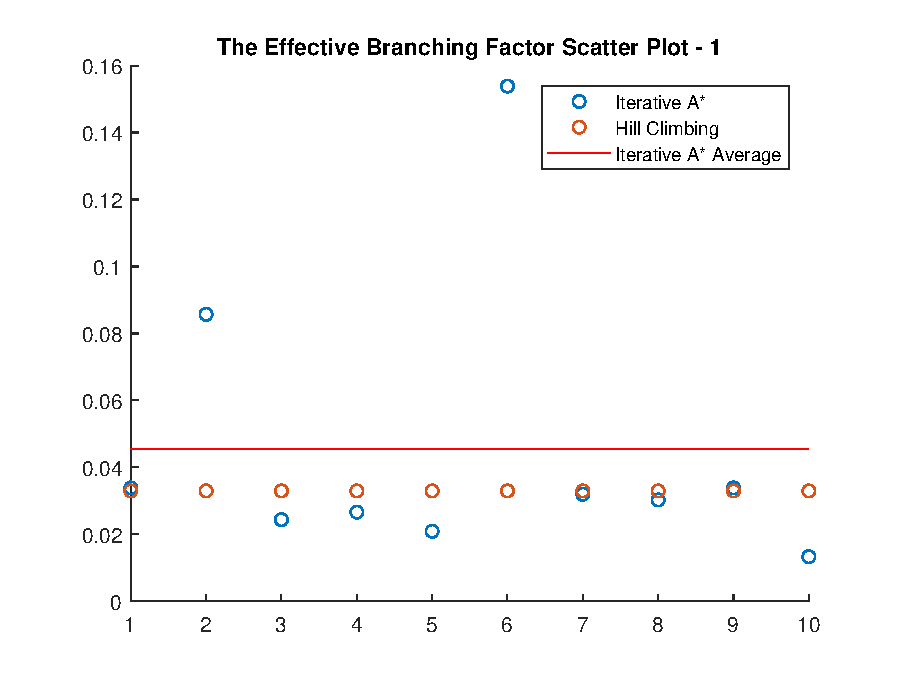
\includegraphics[scale=0.4]{ebf_1}
	\caption{Effective Branch Factor for First F(n)} %
\end{figure}

\paragraph{Alternative function Function F(n)}

However, if we change the function to f(n)=10*(10+attack number) + (10+number of tiles we move2), when we using hill climbing for any 6*6 chess board, the effective factor will be still be 0.03333, which is a constant number. The effective factor of using hill climbing mainly depends on the board size. Thus, we can infer that  using hill climbing to solve a N-Queen problem, the effective factor will be n*(n-1)/1. Whereas, the effective factor of using iterative deepening A* increased to 0.0455 to solve 4*4 boards. 

\begin{figure}[htbp]
	\centering 
	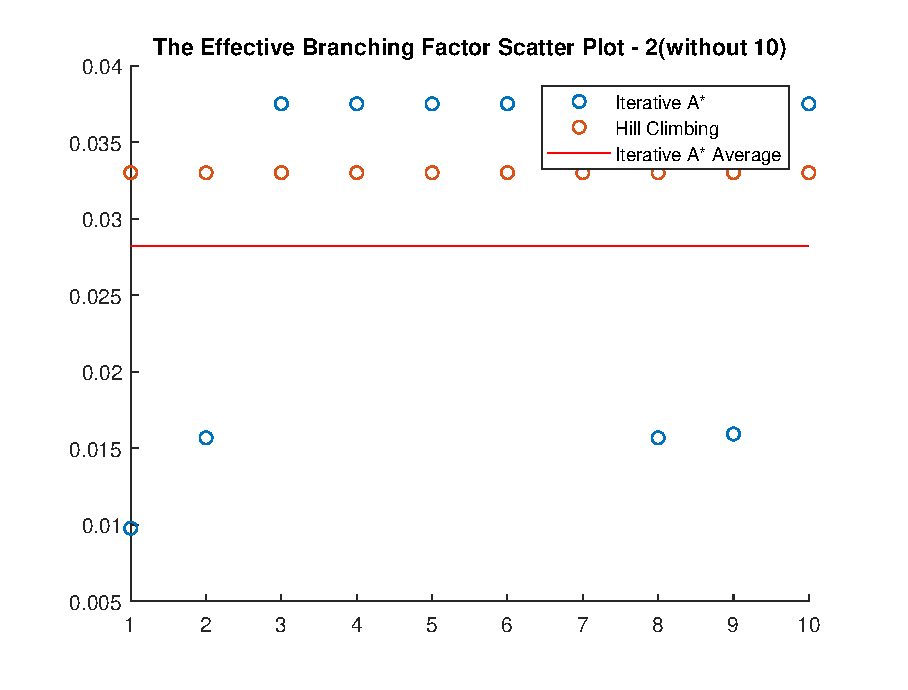
\includegraphics[scale=0.4]{ebf_2}
	\caption{Effective Branch Factor for Second F(n)} %
\end{figure}

\paragraph{Summary}
The reason is because for hill climbing, the program will expand all available node for current state, the number of all the nodes is N*(N-1), and the hill climbing only chooses one node to go, so , the effective factor is a constant value. And for A*, because we changed the heuristic function and added weight to the “h” value. With the new heuristic function, the program is more likely to pick the step that have a lower attack number and is more likely to find the result, when comparing with the old heuristic function. Thus, we can avoid some unnecessary expand when using A*. In consequence, the effective factor of using A* is improved after using the new heuristic function “f(n)=10*(10+attack number) + (10+number of tiles we move2)”.
Our experiment results are shown as follow:



\subsubsection{Cheaper Solutions}

When the number of queens is not very large, hill climbing may come up with a cheaper. However, this situation will change when the number of queens is very large. If the number of queens is very large, the approach of A-star will come up with cheaper solution paths, which will have a lower final cost. Because A-star will explore all the necessary nodes and then only take those nodes that form a most costless path, which is also the global maximum solution. In our program, for A-star, it will pick the next step by calculating f(n)=10*h(n)+g(n), where “h” is the attack number for that step and “g” is the cost for current step plus the cost for all former step it took. However, for greedy hill climbing, f(n)=10*h(n)+g(n), where “g” is the cost for only the current step. This latter approach may lead it take some useless steps, which would increase the final cost for the solution or increase the difficulty to find the true solution. Once hill climbing can’t find a solution in just one chance, it need to restart. All the steps it moved before restart also should be counted into the final cost, even though these steps may fail to find a result. However, in our program, we only output the cost of the final solution path for hill climbing. Thus, we shouldn’t simply compare the output final cost of hill climbing and A*. We should also consider the number of restart. All in all, A-star should come up with a cheaper solution.


\subsubsection{Solutions With Less Time Complexity}


Greedy hill climbing takes much less time than A-star. The reason is because A-star need to expand almost every previous node. The number of expanded nodes increase exponentially. Thus the time complexity for A* is O(bd). However, for hill climbing, the time complexity is O(bd). Thus, A* will take much longer time than hill climbing when the value “N” is very large. We compare the time complexity of hill climbing and A* by running 4 queens, 5 queens, 6 queens and 7 queens each 5 times and take the average running time for each kind of boards. The results are shown as below:

\begin{figure}[htbp]
	\centering 
	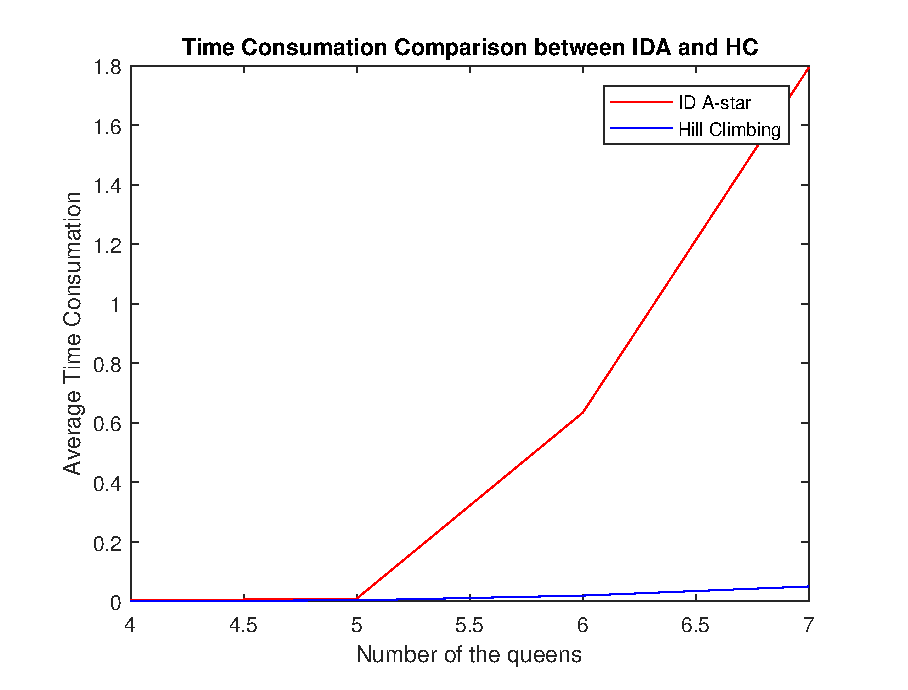
\includegraphics[scale=0.3]{com}
	\caption{Time Consumption Comparison } %
\end{figure}


\section{Urban Planning}

\subsection{Methodology}

For a given map, the first step of both methods is to generate a solution randomly. The solution is a matrix containing the coordinates of different sites and their according type. The matrix is denoted by nested list in Python, the element in the list is a sub-list containing three digits, the first two digits represent the coordinate of the sites and the third digit is the category of the sites, classified by 1, 2 and 3 for industrial, commercial and residential site respectively. 

\subsubsection{Score Calculation}

The score for each solution is calculated depending on the requirement illustrating in the problem part, which is determined the distance between different construction sites, the construction sites and the specific sites on map and the construction cost on different grids. In the program there is a function to calculate the score for each map configuration.
The score will be criteria judging the quality of the solution. The correlation between the score and the solution is positive, the higher score, the better solution. In the hill climbing algorithm, the program is to find the maximum score with the according map configuration; in the genetic algorithm, the fitness is exactly the score.

\subsubsection{Successor Generation}

Hill climbing and genetic algorithm both need to expand nodes to find the optimal solution. The generation of successors is to find all the possible solutions other than the parent solutions. Hill climbing will expand the nodes and choose the best child then expand for next until the peak value is found. In genetic algorithm, a sequence of initial states will be generated then the population will perform random crossover to generate the next population. 


\subsubsection{Hill Climbing}

In the beginning only one possible coordinates sequence will be generated and then the expand nodes for all the other possible solutions. For each iteration, the node with highest score will be chosen to expand nodes. If the score is less than the score than the previous iteration, the program will stop.

\paragraph{Restart}

In the restart process, an estimated upper bound of the score will be given according to the number of sites and the cost of the map. For each iteration, the program will determine whether the highest recorded score is smaller than the estimated score, if it’s smaller than the estimated score, the program continues until the program has ran 10 seconds already. 

\subsubsection{Genetic Algorithm}

In genetic algorithm, the population size and the number of iterations are predetermined value. The population will be random generated at the beginning, then for each iteration, selection, elitism, culling and crossover will be performed to find the optimal solution. 


\subsection{Write Up Question}

\subsubsection{Genetic Algorithm Mechanism}


\subparagraph{Selection}

The selection from a population is to select the individuals according to a probability sequence. The probability is determined by the score of each individual in a certain population. 

In a certain population, the higher score will lead to the higher probability to be fetched. 

\begin{figure}[htbp]
	\centering 
	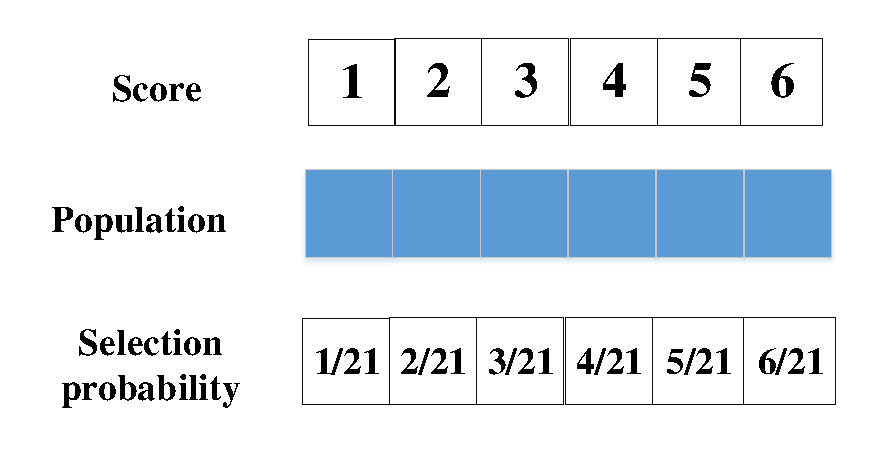
\includegraphics[scale=0.4]{selection}
	\caption{Selection Process} %
\end{figure}

\subparagraph{Crossover}

In this algorithm, crossover is using the the uniform crossover. For the gene segment on the chromosome, choose the segments randomly then perform the crossover.

\begin{figure}[htbp]
	\centering 
	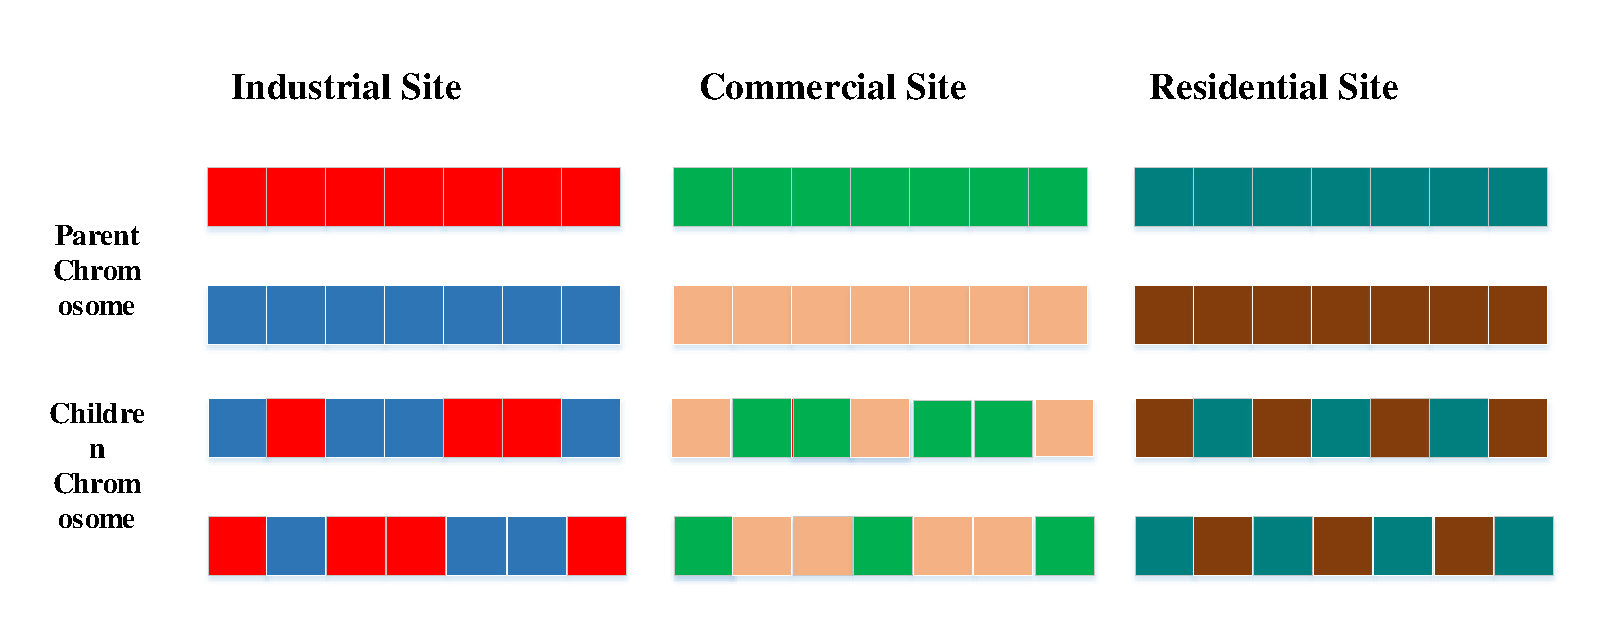
\includegraphics[scale=0.4]{crossover}
	\caption{Crossover Process} %
\end{figure}


\subparagraph{Elitism}

The elitism is performed before the culling and crossover operation. For the population in each iteration, remove the individual with the highest score and keep the individual to next population. 

\begin{figure}[htbp]
	\centering 
	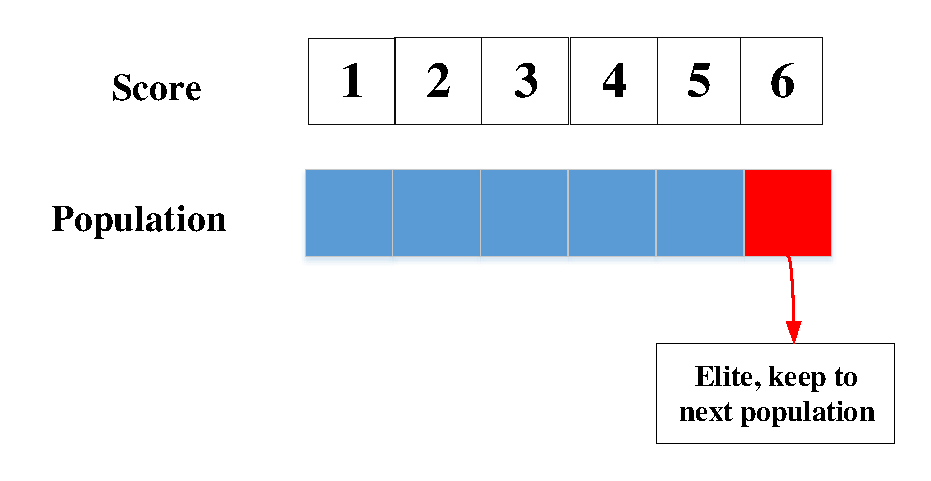
\includegraphics[scale=0.4]{elitism}
	\caption{Elitism Process} %
\end{figure}


\subparagraph{Culling}

The mechanism performs the same as the elitism, which is to remove the element with lowest score. 

\begin{figure}[htbp]
	\centering 
	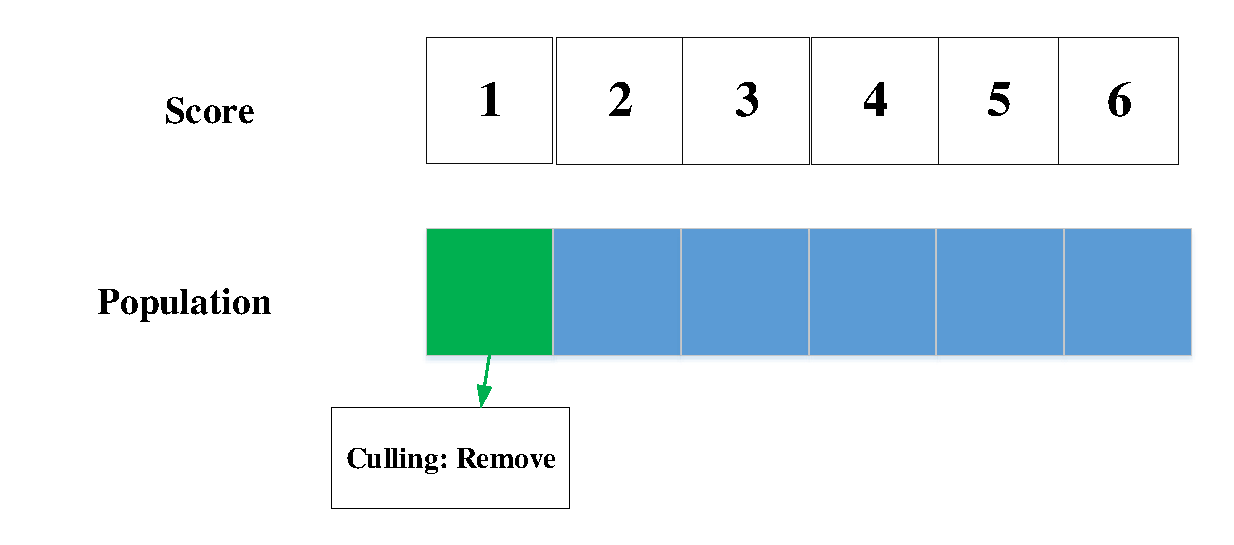
\includegraphics[scale=0.5]{culling}
	\caption{Culling Process} %
\end{figure}


\subparagraph{Mutation}

The mutation will be performed on different sites, which means the different chromosomes will perform their mutations respectively. The segment will mutate randomly.



\subsubsection{Program Performance}

\paragraph{Hill Climbing}


\subparagraph{Without Restart}

This figure illustrated the result of the test map written by our group.

\begin{figure}[htbp]
	\centering 
	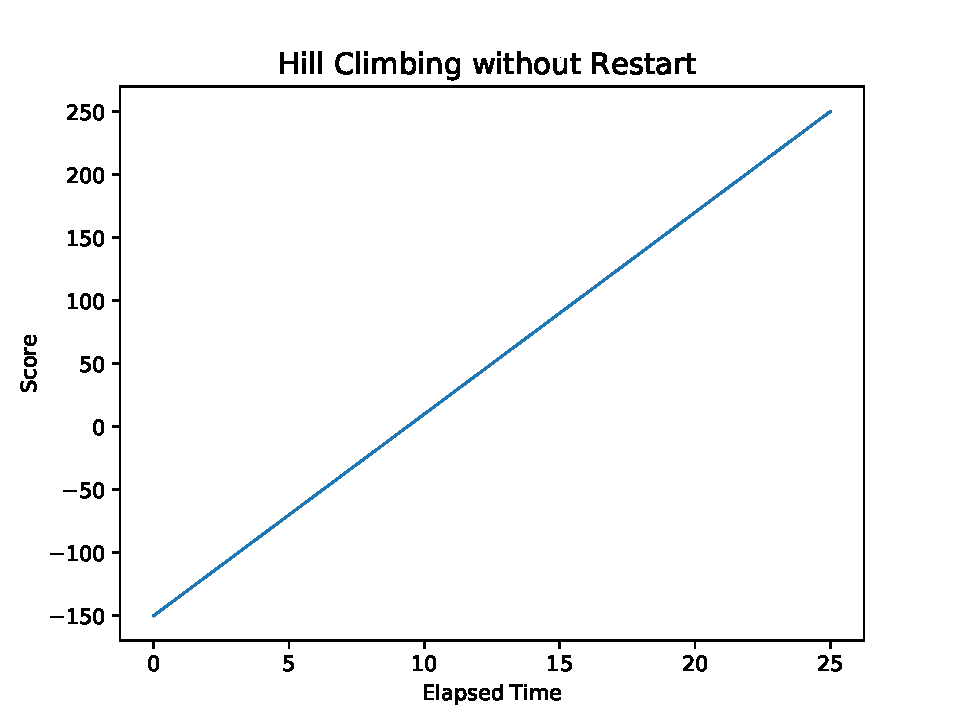
\includegraphics[scale=0.5]{up2_1}
	\caption{Hill Climbing Without Restart} %
\end{figure}

\newpage

\subparagraph{With Restart}

On the following is the result of hill climbing with restart.


\begin{figure}[htbp]
	\centering 
	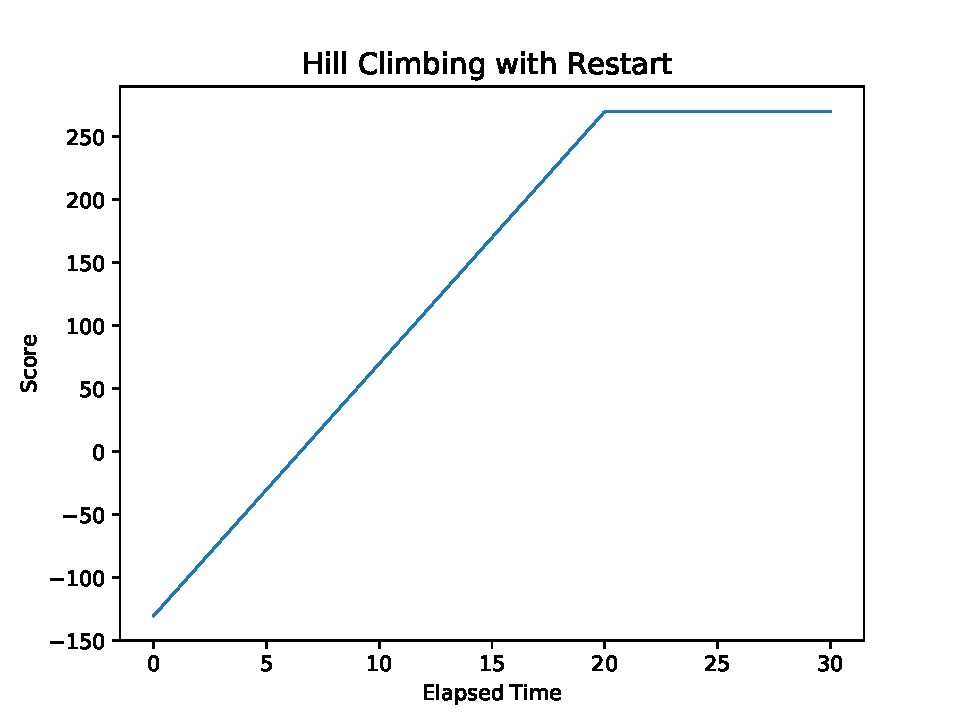
\includegraphics[scale=0.5]{up2_2}
	\caption{Hill Climbing With Restart} %
\end{figure}

\paragraph{Genetic Algorithm}

On the following result is the genetic algorithm with full version.


\begin{figure}[htbp]
	\centering 
	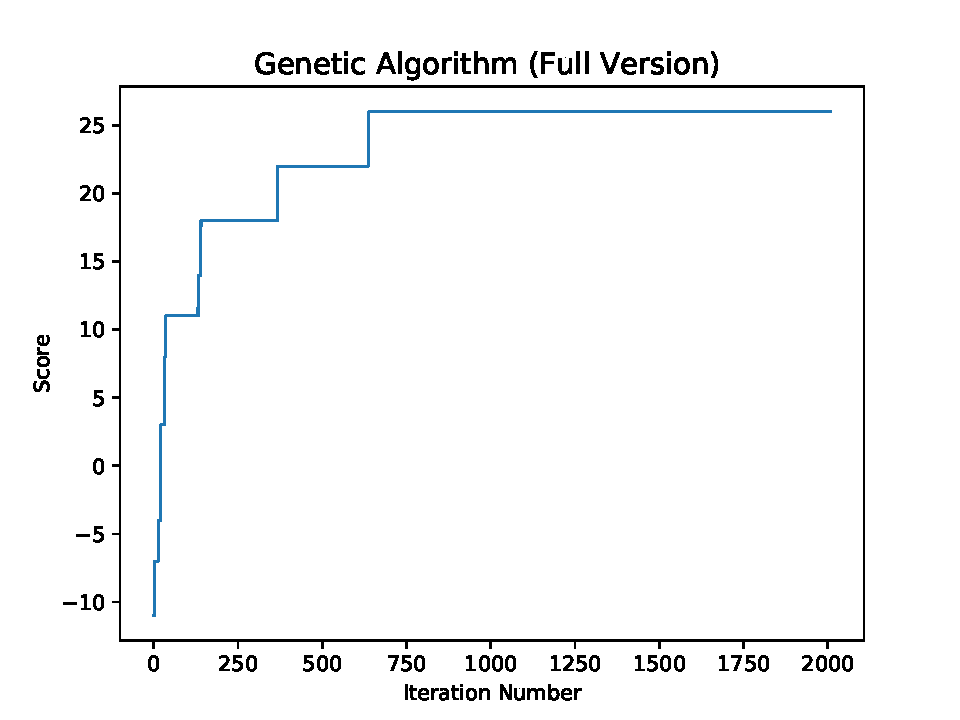
\includegraphics[scale=0.5]{up3_3}
	\caption{Genetic Algorithm} %
\end{figure}

\subsubsection{Effects of Elitism and Culling}

The following figures performed trials on the sample map 2 which is available on Canvas. It demonstrates the full version has better result, to reach higher score in less iterations.


\paragraph{Without Elitism and Culling}

\newpage
\begin{figure}[htbp]
	\centering 
	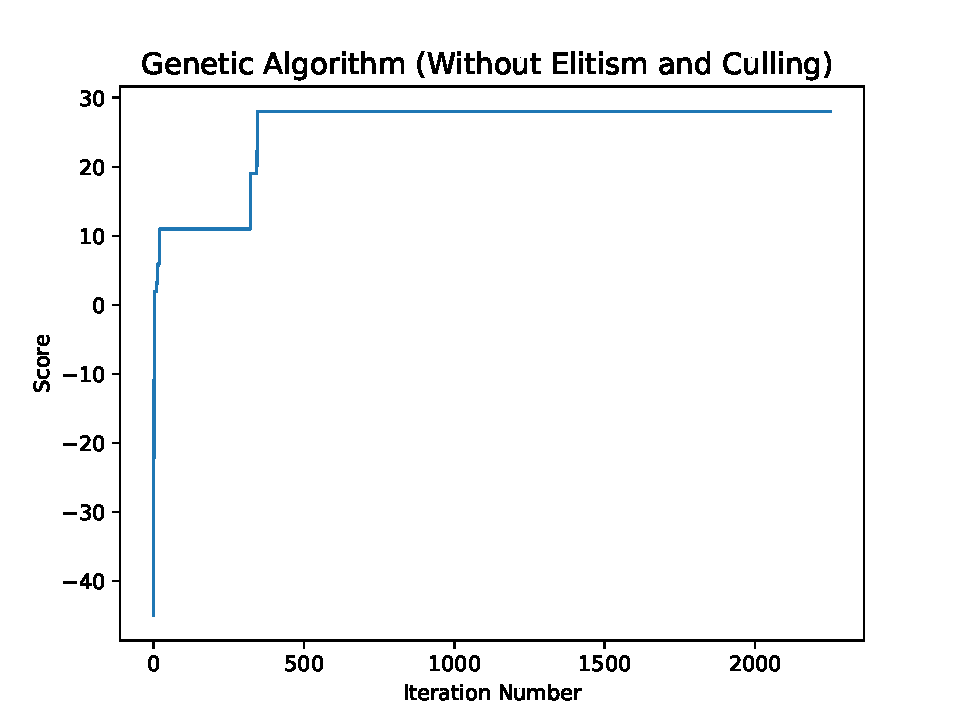
\includegraphics[scale=0.35]{up3_1}
	\caption{Without Elitism and Culling} %
\end{figure}


\paragraph{Without Culling}

The result is on the following:

\begin{figure}[htbp]
	\centering 
	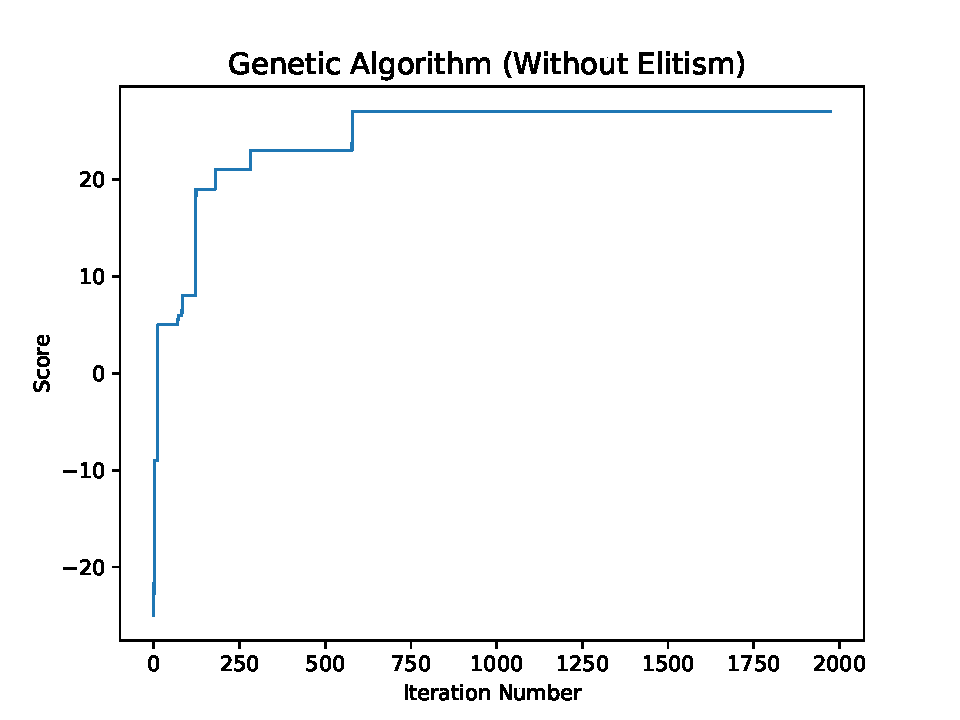
\includegraphics[scale=0.35]{up3_2}
	\caption{Without Culling} %
\end{figure}

\paragraph{Full Version}

The result is on the following:

\begin{figure}[htbp]
	\centering 
	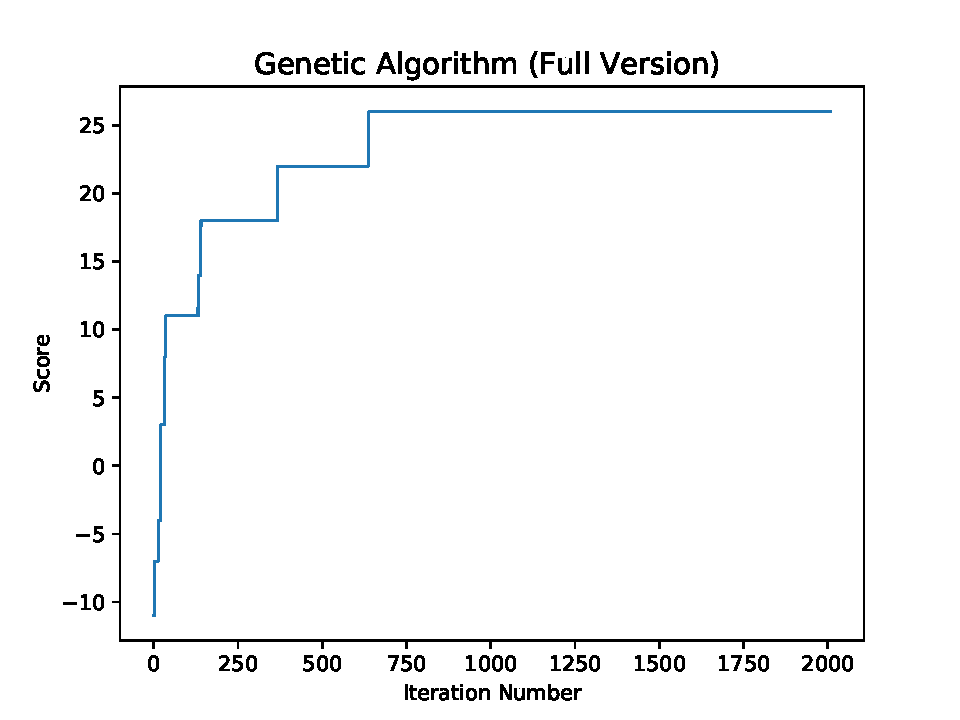
\includegraphics[scale=0.4]{up3_3}
	\caption{Full Version} %
\end{figure}

\subsubsection{Selection and Crossover}

\subparagraph{Perform of Selection}

The selection process is determined by the probability calculated by the score and the sum of all the population. The code implementation is one th following:

\newpage

\begin{lstlisting}
 pop_new = np.asarray(population)
# according to the fitness, perform selection (through index)
index = np.random.choice(np.arange(length), size=length, replace=True, p = scores/scores.sum())
index = index.tolist()
# filter duplicated elements
index = list(set(index))
pop_new = pop_new[index]
\end{lstlisting}


\subparagraph{Perform of Crossover}

The mechanism of the crossover is explained in the writeup question part. 

In the program, the number of the crossover segments will be randomly determined to avoid the generation of same children.

%\tableofcontents

%\listoffigures
%\listoftables
%\lstlistoflistings        


%\newpage




\bibliographystyle{IEEEtran}  
%\bibliography{MyRefs} 
%\addcontentsline{toc}{section}{References}





%-------------------------------------------------------------------------------------------------------





\end{document}
